%===============================================================================
% $Id: ifacconf.tex 19 2011-10-27 09:32:13Z jpuente $  
% Template for IFAC meeting papers
% Copyright (c) 2007-2008 International Federation of Automatic Control
%===============================================================================
\documentclass{ifacconf}

\usepackage{graphicx}      % include this line if your document contains figures
\usepackage{natbib}        % required for bibliography
\usepackage{diffcoeff}
\usepackage{amsmath,amssymb}
\usepackage{bm}
\usepackage{dsfont}
\usepackage{url}
\usepackage{comment}

\makeatletter
\def\endfigure{\end@float}
\def\endtable{\end@float}
\makeatother

\usepackage[caption=false]{subfig}
\usepackage{etoolbox}

\AtBeginEnvironment{figure}{\setlength{\captionwidth}{0.8\linewidth}}
\AtBeginEnvironment{table}{\setlength{\captionwidth}{0.8\linewidth}}
\captionsetup[subfloat]{width=.7\captionwidth}

\newtheorem{remark}{Remark}
\newcommand{\secref}[1]{\S\ref{#1}}

\graphicspath{{./Figures/}}
%===============================================================================
\begin{document}
\begin{frontmatter}

\title{Partitioned finite element method for power-preserving structured discretization with mixed boundary conditions\thanksref{footnoteinfo}} 
% Title, preferably not more than 10 words.

\thanks[footnoteinfo]{This work is  supported by the project ANR-16-CE92-0028,
	entitled {\em Interconnected Infinite-Dimensional systems for Heterogeneous
		Media}, INFIDHEM, financed by the French National
	Research Agency (ANR) and the Deutsche Forschungsgemeinschaft (DFG). Further information is available at {\url{https://websites.isae-supaero.fr/infidhem/the-project}}.}

\author[ISAE]{Andrea Brugnoli} 
\author[ITA]{Fl\'avio Luiz Cardoso-Ribeiro} 
\author[ISAE]{Ghislain Haine}
\author[TUM]{Paul Kotyczka}

\address[ISAE]{ISAE-SUPAERO, Universit\'e de Toulouse,
	10 Avenue Edouard Belin, BP-54032, 31055 Toulouse Cedex 4, France
	(e-mail: \{andrea.brugnoli, ghislain.haine\}@isae.fr).}
\address[ITA]{Instituto Tecnol\'ogico de Aeron\'autica, Brazil (e-mail:flaviocr@ita.br).}
\address[TUM]{Chair of Automatic Control, Technical University of Munich, 85748 Garching, Germany (e-mail:kotyczka@tum.de).}

\begin{abstract}                % Abstract of not more than 250 words.
The propagation of acoustic waves in a 2D geometrical domain under mixed boundary control is here described by means of the port-Hamiltonian (pH) formalism. A finite element based method is employed to obtain a consistently discretized model. To construct a model with mixed boundary control, two different methodologies are detailed: one employs Lagrange multipliers, the other relies on a virtual domain decomposition to interconnect models with different causalities. The two approaches are assessed numerically, by comparing the Hamiltonian and the state variables norm for progressively refined meshes.
\end{abstract}

\begin{keyword}
Aeroacoustics, port-Hamiltonian systems (pHs), Partitioned Finite Element Method (PFEM), Mixed Boundary Control.
\end{keyword}

\end{frontmatter}
%===============================================================================


\section{Introduction}
The port-Hamiltonian (pH) formalism has demonstrated to be a valuable modelling paradigm, capable of highlighting important properties of dynamical systems (\cite{bookPHs}) and representing a huge class of systems, either finite- or infinite-dimensional (\cite{VANDERSCHAFT2002}). Obtaining finite-dimensional representations that preserve the proprieties of the continuous system at a discrete level is not a trivial task. Many techniques (e.g. \cite{moulla:hal-01625008}) are only applicable to one-dimensional problems and cannot treat higher geometrical dimensions. Finite differences (\cite{Trenchant}) can be used for 2D problems but the actual implementation cannot be automated easily. A finite element approach dealing with different boundary causality has been proposed in \cite{WeakForm_Kot}. The construction of the necessary power-preserving mappings is, however, not straightforward on arbitrary meshes. \\

The method of choice for this paper is detailed in \cite{cardoso2019partitioned}. It represents the extension of the mixed finite element method (\cite{Gatica}) to pH systems and as such it can be easily implemented using standard finite elements libraries (e.g. \cite{LoggMardalEtAl2012}). Because of the different treatment of the system equations, which allows the choice of imposed boundary conditions, this method is referred to as partitioned finite element method (PFEM). Despite the many advantages of PFEM, the inclusion of mixed boundary conditions demands additional care. A detailed discussion, both at a theoretical and numerical level, on mixed boundary control problems in 2D geometric domains may be found in~\cite{Grisvard}.\\

In this work, the propagation of acoustic waves in a cylindrical duct is considered. An analogous problem and its discretization are studied in \cite{WU2015206}. To illustrate how mixed boundary control are handled in PFEM, an impedance boundary condition is taken over the lateral surface of the cylinder, whereas on the remaining boundary a constant flux is imposed at the inlet and the outlet. Two different methodologies to treat the mixed boundary causalities are detailed and numerically compared.   \\

In Section \ref{sec:model} the problem under consideration is detailed. The boundary and initial conditions are assumed to be axis-symmetric. This allows reducing the problem from a 3D to a 2D geometry. In Section \ref{sec:PFEM} the partitioned finite element method is recalled, under the hypothesis of uniform boundary conditions. In Section \ref{sec:mixed_bc} the treatment of mixed boundary conditions is described. One strategy relies on the usage of Lagrange multipliers to enforce the Dirichlet boundary condition. The other requires the constructions of two models with different causality by splitting the domain into two parts. These two models are then interconnected to get a final system with mixed boundary inputs. In Sections \ref{sec:numerics} the numerical simulations provided by the two different methods are presented. By progressively refining the mesh size, it is shown that, for both methods, the states converge to the results of a reference solution.

\section{Problem statement: model description}
\label{sec:model}
In this section we state the problem under consideration by making use of a port-Hamiltonian model. The reader can consult \cite{BookZwart} for a comprehensive introduction to 1D distributed parameter PH systems and links towards classical PDE models. The canonical PH representation of hyperbolic conservation laws in nD is presented in \cite{VANDERSCHAFT2002}.

The propagation of sound in air inside  is modeled by \cite{Trenchant}
\begin{equation}
\label{eq:gen_mod}
    \diffp{}{t}
    \begin{bmatrix}
    \chi_s p \\
    \mu_0 \bm{v} \\
    \end{bmatrix} = -
    \begin{bmatrix}
    0 & \mathrm{div} \\
    \mathrm{grad} & 0 \\
    \end{bmatrix}
    \begin{bmatrix}
    p \\
    \bm{v} \\
    \end{bmatrix},
\end{equation}
on $\Omega \subset \mathbb{R}^3$. $p \in \mathbb{R}$  and $\bm{v} \in \mathbb{R}^3$ denote the variations of pressure and velocity from a steady state, $\mu_0$ is the steady state mass density, and $\chi_s$ represents a constant adiabatic compressibility factor.  A cylindrical duct of length $L$ and radius $R$ is considered as physical domain, $\Omega = \{x \in [0, L], r \in [0, R], \theta = [0, 2 \pi)\}$. Denoting by $x, r, \theta$ the axial, radial and tangential coordinate,  the following boundary conditions are imposed
\begin{align}
    p(x, R, \theta) &= - \mathcal{Z}(x, t) \, v_r(x, R, \theta), \label{eq:bc_imp} \\
    \bm{v} \cdot \bm{n}(0, r, \theta) &= -v_x(0, r, \theta) = - f(r), \label{eq:bc_flowL}\\
    \bm{v} \cdot \bm{n}(L, r, \theta) &= +v_x(L, r, \theta) = + f(r), \label{eq:bc_flowR}
\end{align}
where $\bm{n}$ is the outward normal at the boundary. As the main focus is the treatment of mixed boundary conditions, it is assumed that the impedance operator $\mathcal{Z}$ is non invertible. If it were invertible than the impedance condition could be treated as a Robin condition. For the initial boundary conditions, it is assumed
\begin{equation}
\label{eq:init_con}
\begin{aligned}
    p^0(x, r, \theta) &= 0, \\
    v_x^0(x, r, \theta) &= f(r), 
\end{aligned}  \qquad
\begin{aligned}
    v_r^0(x, r, \theta) &= g(r), \\
    v_\theta^0(x, r, \theta) &= 0.
\end{aligned}    
\end{equation}
The impedance and the axial and radial flows expressions are the following
\begin{equation*}
\begin{aligned}
\mathcal{Z}(x, t) &= \mathds{1}\left\{ \frac{1}{3} L \leq \ x \ \leq \frac{2}{3} L, \,  t \geq 0.2 \ t_{\text{fin}} \right\} \mu_0 \, c_0, \\
f(r) &= \left( 1 - \frac{r^2}{R^2} \right) v_0, \\
g(r) &= 16 \frac{r^2}{R^4} \left( R - r \right)^2 v_0. \\
\end{aligned}
\end{equation*}
 This model describes the behavior of an axis-symmetrical flow subjected to an impedance condition on the lateral surface. Because of symmetry the model can be reduced to a 2D problem in polar coordinates over the domain $\Omega_{\text{r}} = \{x \in [0, L], r \in [0, R]\}$. The reduced system reads
\begin{equation}
\label{eq:red_mod}
    \diffp{}{t}
    \begin{bmatrix}
    \chi_s p \\
    \mu_0 v_x \\
    \mu_0 v_r \\
    \end{bmatrix} = -
    \begin{bmatrix}
    0 & \partial_x & \partial_r + 1/r \\
    \partial_x & 0 & 0 \\
    \partial_r & 0 & 0 \\
    \end{bmatrix}
    \begin{bmatrix}
    p \\
    v_x \\
    v_r \\
    \end{bmatrix}.
\end{equation}
The boundary conditions must now account for the symmetry condition at $r=0$, leading to the additional condition $\bm{v}\cdot \bm{n}(x, 0) = v_r(x, 0) =0$. System \eqref{eq:red_mod} can be rewritten compactly as a pH system in co-energy variables 
\begin{equation}
\label{eq:sys_ph}
    \mathcal{Q}^{-1} \partial_t{e} = \mathcal{J} e
\end{equation}
where $\mathcal{Q}^{-1} = \mathrm{diag}([\chi_s, \ \mu_0, \ \mu_0])$ is a bounded, coercive operator and $e = [p, \ v_x, \ v_r]$ is the vector of the co-energy variables. The Hamiltonian is then computed as
\[
H = \frac{1}{2} \left(e, \mathcal{Q}^{-1} e  \right)_{\Omega_{\text{r}}}
\]
where $\left(\cdot, \cdot \right)_{\Omega_{\text{r}}}$ is the standard $L^2$ inner product in polar coordinates
\[
\left(\alpha, \beta \right)_{\Omega_{\text{r}}} = \int_{\Omega_{\text{r}}} \alpha \cdot \beta \ r \d{r} \d{x} = \int_{\Omega_{\text{r}}} \alpha \cdot \beta \ \d{\Omega_r}.
\]
The power flow is obtained by application of the Stokes theorem
\[
\dot{H} = \int_{\partial \Omega_{\text{r}}} p \ \bm{v} \cdot \bm{n} \d{\Gamma_r} = - \int_{0}^{L} \mathcal{Z}(x, t) v_r^2 \ R \d{x} \le 0 
\]
where $\d{\Gamma_r} = r \d{s}$ is the infinitesimal surface. The interconnection operator $\mathcal{J}$ can be decomposed in the sum of $\mathcal{J} = \mathcal{J}_{\text{div}} + \mathcal{J}_{\text{grad}}$
\begin{equation}
\label{eq:J_dec}
    \mathcal{J}_{\text{div}} = -\begin{bmatrix}
    0 & \partial_x & \partial_r + 1/r \\
    0 & 0 & 0 \\
    0 & 0 & 0 \\
    \end{bmatrix}, \qquad 
    \mathcal{J}_{\text{grad}} = -\begin{bmatrix}
    0 & 0 & 0 \\
    \partial_x & 0 & 0 \\
    \partial_r & 0 & 0 \\
    \end{bmatrix}.
\end{equation}
Such a decomposition is meaningful as $\mathcal{J}_{\text{grad}}^* = -\mathcal{J}_{\text{div}}$, where $^*$ denote the formal adjoint operator and it is especially useful to illustrate the partitioned finite element method. 

\section{Recall on the Partitioned Finite Element Method}
\label{sec:PFEM}
In this section the partitioned finite element method \cite{cardoso2019partitioned} is recalled by considering uniform (either Neumann or Dirichlet in standard terminology) boundary conditions. The idea boils down to three simple steps:
\begin{enumerate}
	\item write the system in weak form;
	\item perform integration by parts to one part of the equations to get the chosen boundary control;
	\item select the finite element spaces to achieve a finite-dimensional system.
\end{enumerate}
The second step is crucial as it determines which boundary condition appears as input, defining the causality of the system.  The weak form is obtained by considering the scalar product of system \eqref{eq:sys_ph} against a test function $w=[w_p, \ w_{vx}, \ w_{vy}]=[w_p, \ \bm{w}_{v}]$ 
\begin{equation}
\label{eq:weak_form}
    \left(w, \mathcal{Q}^{-1} \partial_t{e} \right)_{\Omega_{\text{r}}} = \left(w, \mathcal{J} e \right)_{\Omega_{\text{r}}}.
\end{equation}
As $Q$ is coercive the inner product on the left hand side corresponds to a symmetric and coercive bilinear form 
\[m(w, \partial_t{e}) := \left(w, \mathcal{Q}^{-1} \partial_t{e} \right)_{\Omega_{\text{r}}}.
\]
The integration by parts will define which boundary control will appear explicitly.

\subsection{Neumann boundary control}
\label{sec:neu_bc}
If the integration by parts is applied on $\mathcal{J}_{\text{div}}$ then the right hand-side of Eq. \eqref{eq:weak_form} becomes
\begin{equation*}
    \left(w, \mathcal{J} e \right)_{\Omega_{\text{r}}} = \left(w, \mathcal{J}_{\text{grad}} \ e \right)_{\Omega_{\text{r}}} - \left(\mathcal{J}_{\text{grad}} \ w, e \right)_{\Omega_{\text{r}}} + \left(w_p, u_N \right)_{\partial \Omega_{\text{r}}}.
\end{equation*}
The skew-symmetric bilinear form 
\[ j_{\text{grad}}(w, e) := \left(w, \mathcal{J}_{\text{grad}} \ e \right)_{\Omega_{\text{r}}} - \left(\mathcal{J}_{\text{grad}} \ w, e \right)_{\Omega_{\text{r}}} \]
may now be introduced, together with the boundary form
\begin{equation}
\label{eq:f_N}
 \left(w_p, u_N \right)_{\partial \Omega_{\text{r}}} = \int_{\partial \Omega_{\text{r}}} w_p u_N \ \d{\Gamma_r},
\end{equation}
where $u_N = \bm{v} \cdot \bm{n} \vert_{\partial \Omega_r}$. The corresponding power conjugated output is given by $y_N = p \vert_{\partial \Omega_r}$. The output is then discretized considering the scalar test function $w_N$ defined only over the boundary $\partial \Omega_r$. The system in weak form under Neumann boundary control is then written as
\begin{equation}
\label{eq:wf_grad}
\begin{aligned}{}
m(w, \partial_t{e}) &= j_{\text{grad}}(w, e) + \left(w_p, u_N \right)_{\partial \Omega_{\text{r}}}. \\
\left(w_N, y_N \right)_{\partial \Omega_{\text{r}}} &= \left(w_N, p \right)_{\partial \Omega_{\text{r}}},
\end{aligned}
\end{equation}

\subsection{Dirichlet boundary control}
\label{sec:dir_bc}
If the integration by parts is carried out on $\mathcal{J}_{\text{grad}}$ then the right hand-side of \eqref{eq:weak_form} becomes
\begin{equation*}
    \left(w, \mathcal{J} e \right)_{\Omega_{\text{r}}} = \left(v, \mathcal{J}_{\text{div}} \ e \right)_{\Omega_{\text{r}}} - \left(\mathcal{J}_{\text{div}} \ w, e \right)_{\Omega_{\text{r}}} + \left(\bm{w}_v \cdot \bm{n}, u_D \right)_{\partial \Omega_{\text{r}}}.
\end{equation*}
The skew-symmetric bilinear form 
\[ j_{\text{div}}(w, e) := \left(w, \mathcal{J}_{\text{div}} \ e \right)_{\Omega_{\text{r}}} - \left(\mathcal{J}_{\text{div}} \ w, e \right)_{\Omega_{\text{r}}} \]
is introduced, together with the boundary form
\begin{equation}
\left(\bm{w}_v \cdot \bm{n}, u_D \right)_{\partial \Omega_{\text{r}}} = \int_{\partial \Omega_{\text{r}}} \bm{w}_v \cdot \bm{n} \ u_D \ \d{\Gamma_r}, 
\end{equation}
where $u_D = p \ \vert_{\partial \Omega_r}$. Adding  the conjugated output $y_D = \bm{v}\cdot~\bm{n}\vert_{\partial \Omega_r}$, the system in weak form under Dirichlet boundary control is then written as
\begin{equation}
\label{eq:wf_div}
\begin{aligned}
m(w, \partial_t{e}) &= j_{\text{div}}(w, e) + \left(\bm{w}_v \cdot \bm{n}, u_D \right)_{\partial \Omega_{\text{r}}}, \\
\left(w_D, y_D \right)_{\partial \Omega_{\text{r}}} &= \left(w_D, \bm{v}\cdot\bm{n} \right)_{\partial \Omega_{\text{r}}},
\end{aligned}
\end{equation}
where $w_D$ are scalar test function defined only over the boundary $\partial \Omega_r$.
\section{Extension for Mixed Boundary Conditions}
\label{sec:mixed_bc}
In this section we consider the case in which Neumann and Dirichlet boundary control co-exist. The partitioned finite element method allows to treat this case by means of two different approaches. One relies on a differential-algebraic formulation, the other on a purely differential formulation by exploiting a classical interconnection of pH systems together with a domain decomposition.

\subsection{Lagrange Multipliers}
\label{sec:lgr_mul}
This approach can equivalently use Eq. \eqref{eq:wf_grad} or Eq. \eqref{eq:wf_div} as a starting point. The weak form \eqref{eq:wf_grad} will be used both for the illustration of the method and for numerical computations. 
\begin{figure}[t]%
	\centering
	\includegraphics[width=0.65\columnwidth]{boundary_part.eps} \\
	\caption[bcpart]{Boundary partition for the problem.}
	\label{fig:bc_part}
\end{figure}
The boundary is split in two partition (see Fig. \ref{fig:bc_part}). For the time being generic inputs $u_D, u_N$ for the Dirichlet and Neumann conditions are considered.  First of all the boundary term in Eq. \eqref{eq:f_N} needs to be revisited. The quantity $\bm{v}\cdot\bm{n}\vert_{\partial \Omega_{\text{r}}}$ is known only $\Gamma_N$. On $\Gamma_D$ a Lagrange multiplier $\lambda_D$ has to be introduced to enforce the Dirichlet boundary condition. This leads to 
\begin{equation}
\label{eq:bdint_dae}
\int_{\partial \Omega_{\text{r}}} w_p \bm{v} \cdot \bm{n} \d{\Gamma_r} = \int_{\Gamma_N} w_p u_N \ \d{\Gamma_r} + \int_{\Gamma_D} w_p \lambda_D \d{\Gamma_r}.
\end{equation}
The constraint associated with the Lagrange multiplier  is the in-homogeneous Dirichlet condition
\begin{equation}
\label{eq:wf_con}
\int_{\Gamma_D} w_\lambda (p - u_D) \d{\Gamma_r} = 0,
\end{equation}
where $w_\lambda$ is the test function associated with the Lagrange multiplier. The system in weak form is obtained by using Eqs. \eqref{eq:wf_grad}, \eqref{eq:f_N}, \eqref{eq:bdint_dae} and \eqref{eq:wf_con}, together with the power conjugated outputs ($y_N = p|_{\Gamma_N}, \; y_N = \lambda_D|_{\Gamma_D} = \bm{v} \cdot \bm{n}|_{\Gamma_D}$)
\begin{equation}
\begin{aligned}
m(w, \partial_t{e}) &= j_{\text{grad}}(w, e) + \left(w_p, u_N \right)_{\Gamma_N} + \left(w_p, \lambda_D \right)_{\Gamma_D}, \\
0 &= - \left(w_\lambda, p \right)_{\Gamma_D} + \left(w_\lambda, u_D \right)_{\Gamma_D}, \\
\left(w_N, y_N \right)_{\Gamma_N} &= \left(w_N, p \right)_{\Gamma_N}, \\
\left(w_D, y_D \right)_{\Gamma_D} &= \left(w_D, \lambda_D \right)_{\Gamma_D}, 
\end{aligned}
\end{equation}
where $w_N, w_D$ are the test functions associated to the output discretization and $\left( \cdot, \cdot \right)_{\Gamma_{*}}$ is the $L^2$ inner product on boundary $\Gamma_*$. A Galerkin method can now be applied to retrieve a finite dimensional pH system. This means that corresponding test and trial functions are discretized using the same basis
\begin{align*}
\begin{aligned}
e &\approx \bm\phi_e \mathbf{e}, \\
p &\approx \bm\phi_p \mathbf{p}
\end{aligned} \qquad
\begin{aligned}
\lambda_D/u_D/y_D &\approx \bm\phi_D \bm{\lambda}_D/\mathbf{u}_D/\mathbf{y}_D, \\
y_N &\approx \bm\phi_N \mathbf{u}_N
\end{aligned}
\end{align*}

 leading to the finite dimensional pHDAE (\cite{beattie2018linear}):
\begin{equation}
\begin{aligned}
\label{eq:discr_phdae}
\begin{bmatrix}
\mathbf{M} & \mathbf{0} \\
\mathbf{0} & \mathbf{0} \\
\end{bmatrix} \frac{\d}{\d t}
\begin{bmatrix}
\mathbf{e}\\
\bm{\lambda}_D \\
\end{bmatrix}
&= \begin{bmatrix}
\mathbf{J} & \mathbf{G}_D\\
-\mathbf{G}_D^T & \mathbf{0} \\
\end{bmatrix}
\begin{bmatrix}
\mathbf{e}\\
\bm{\lambda}_D \\
\end{bmatrix} + \begin{bmatrix}
\mathbf{B}_N & \mathbf{0}\\
\mathbf{0} & \mathbf{B}_D \\
\end{bmatrix}
\begin{bmatrix}
\mathbf{u}_N \\
\mathbf{u}_D \\
\end{bmatrix}, \\
\begin{bmatrix}
\mathbf{y}_N \\
\mathbf{y}_D \\
\end{bmatrix} &=
\begin{bmatrix}
\mathbf{B}_N^T & \mathbf{0} \\ 
\mathbf{0} & \mathbf{B}_D^T \\ 
\end{bmatrix}
\begin{bmatrix}
\mathbf{e}\\
\bm{\lambda}_D \\
\end{bmatrix}.
\end{aligned}
\end{equation}
where 
\begin{equation*}
\begin{aligned}
\mathbf{M}^{ij} &= m({\phi}_{e}^i, {\phi}_{e}^j), \\
\mathbf{J}^{ij} &= j_{\text{grad}}({\phi}_{e}^{i}, {\phi}_{e}^{j}), \\
\mathbf{G}_{D}^{ij} &= ({\phi}_{p}^i, {\phi}_{D}^j)_{\Gamma_D}, 
\end{aligned} \qquad 
\begin{aligned}
\mathbf{B}_{N}^{ij} &= ({\phi}_{p}^{i}, {\phi}_{N}^{j})_{\Gamma_N}, \\ \mathbf{B}_{D}^{ij} &= ({\phi}_{p}^{i}, {\phi}_{N}^{j})_{\Gamma_N}. 
\end{aligned}\\
\end{equation*}
\begin{remark}
The output vector $\mathbf{y}_N, \mathbf{y}_D$ does not correspond to the actual degrees of freedom. In fact it has been defined incorporating the boundary mass matrix $\mathbf{M}_{\Gamma_N}, \, \mathbf{M}_{\Gamma_D}$. The actual degrees of freedom corresponding to the output are found by solving
\begin{equation}
\label{eq:y_dof}
\begin{bmatrix}
\mathbf{M}_{\Gamma_N} & \mathbf{0} \\
\mathbf{0} & \mathbf{M}_{\Gamma_D} \\
\end{bmatrix}
\begin{bmatrix}
\widehat{\mathbf{y}}_N \\
\widehat{\mathbf{y}}_D \\
\end{bmatrix} = 
\begin{bmatrix}
\mathbf{y}_N \\
\mathbf{y}_D \\
\end{bmatrix}, \qquad
\mathbf{M}_{\partial\Omega_r} \,  \widehat{\mathbf{y}} = \mathbf{y}.
\end{equation}
However, this definition of output is in accordance with the classical power balance for finite-dimensional pH systems
\begin{align*}
\dot{H} &= \int_{\Gamma_N} u_N y_N \d{\Gamma_N} + \int_{\Gamma_D} u_D y_D \d{\Gamma_D} \\
&\approx \mathbf{u}_N^T \mathbf{M}_{\Gamma_N} \widehat{\mathbf{y}}_N + \mathbf{u}_D^T \mathbf{M}_{\Gamma_D} \widehat{\mathbf{y}}_D = \mathbf{u}_N^T \mathbf{y}_N + \mathbf{u}_D^T \mathbf{y}_D.
\end{align*}
The actual degrees of freedom will be used in \secref{sec:vdd} to get the proper interconnection when connecting systems with different causality.
\end{remark}

Concerning the actual boundary conditions, on $\Gamma_D$ the impedance condition \eqref{eq:bc_imp} is applied while on  $\Gamma_N$ the inlet and outlet flow condition \eqref{eq:bc_flowL}, \eqref{eq:bc_flowR} hold on the left and right side of the rectangle. The impedance boundary conditions is imposed by putting into weak form the expression $u_D=-\mathcal{Z}\lambda_D=-\mathcal{Z}y_D$:
\[ \mathbf{M}_{\Gamma_D} \mathbf{u}_D = - \mathbf{M}_{\Gamma_D, \mathcal{Z}} \widehat{\mathbf{y}}_D,
\]
where $\mathbf{M}_{\Gamma_D, \mathcal{Z}}$ corresponds to the mass matrix associated to the weighted inner product $\left(w_D, \mathcal{Z}  y_D\right)_{\Gamma_D}$, namely $\mathbf{M}_{\Gamma_D, \mathcal{Z}}^{ij} = \left(\phi_D^i, \mathcal{Z}  \phi_D^j \right)_{\Gamma_D}$. This amounts to applying to system \eqref{eq:sys_dae} the control law
\[ \mathbf{u}_D = - \mathbf{M}_{\Gamma_D}^{-1} \mathbf{M}_{\Gamma_D, \mathcal{Z}} \mathbf{M}_{\Gamma_D}^{-1} \mathbf{y}_D = -\mathbf{Z} \mathbf{y}_D.
\]
The Neumann boundary condition is imposed by projection on the $u_N$ space.   The boundary controlled system becomes   
\begin{equation}
\label{eq:sys_dae}
\begin{bmatrix}
\mathbf{M} & \mathbf{0} \\
\mathbf{0} & \mathbf{0} \\
\end{bmatrix} \frac{\d}{\d t}
\begin{bmatrix}
\mathbf{e}\\
\bm{\lambda}_D \\
\end{bmatrix}
= \begin{bmatrix}
\mathbf{J} & \mathbf{G}_D\\
-\mathbf{G}_D^T & -\mathbf{R} \\
\end{bmatrix}
\begin{bmatrix}
\mathbf{e}\\
\bm{\lambda}_D \\
\end{bmatrix} + \begin{bmatrix}
\mathbf{b}_N \\
\mathbf{0} \\
\end{bmatrix},
\end{equation}
with $\mathbf{R} = \mathbf{B}_D \mathbf{Z} \mathbf{B}_D^T$ a symmetric positive definite matrix. 

\subsection{Virtual Domain Decomposition}
\label{sec:vdd}
In order to apply this methodology the domain has to be split into two sub-domains. The shared boundary connecting the two sub-domains can be freely chosen. For the given geometry, the separation line that provide the most regular simplicial meshes is the trapezoidal one given in Fig. \ref{fig:dom_dec}. 
\begin{figure}[t]%
	\centering
	\includegraphics[width=0.65\columnwidth]{domain_split.eps} \\
	\caption{Virtual decomposition of the domain.}
	\label{fig:dom_dec}
\end{figure}
Starting from the PDE \eqref{eq:sys_ph} two weak formulations are constructed: one integrating over $\Omega_N$, the other over $\Omega_D$:
\begin{align}
    \left(w, \mathcal{Q}^{-1} \partial_t{e} \right)_{\Omega_N} = \left(w, \mathcal{J} e \right)_{\Omega_{N}} \label{eq: wf_OmN}, \\
    \left(w, \mathcal{Q}^{-1} \partial_t{e} \right)_{\Omega_D} = \left(w, \mathcal{J} e \right)_{\Omega_{D}}, \label{eq: wf_OmD}
\end{align}

Then, Eqs. \eqref{eq: wf_OmN}, \eqref{eq: wf_OmD} are manipulated according to \secref{sec:neu_bc}, \secref{sec:dir_bc}, respectively:
\begin{equation}
\label{eq:wfdec_intbp}
\begin{aligned}
m^{\Omega_N}(w, \partial_t{e}) &= j_{\text{grad}}^{\Omega_N}(w, e) + \left(w_p, u_N \right)_{\partial \Omega_N}, \\
m^{\Omega_D}(w, \partial_t{e}) &= j_{\text{div}}^{\Omega_D}(w, e) + \left(\bm{w}_v \cdot \bm{n}, u_D \right)_{\partial \Omega_D}, \\
\end{aligned}
\end{equation}
where $\partial \Omega_{N/D}$ denotes the boundary of each sub-domain and the superscript ${\Omega_{N,D}}$ denote that the bilinear forms are obtained by integration over each sub-domain
\[
j_{\text{div/grad}}^{\Omega_{N/D}}(w, e) := \left(w, \mathcal{J}_{\text{div/grad}}  e \right)_{\Omega_{N/D}} - \left(\mathcal{J}_{\text{div/grad}}  w, e \right)_{\Omega_{N/D}}.
\]
The boundary terms in \eqref{eq:wfdec_intbp} are then split into two contributions $\partial\Omega_N = \Gamma_N \cup \Gamma_{\text{int}}, \; \partial\Omega_D = \Gamma_D \cup \Gamma_{\text{int}}$ so that the common boundary is highlighted
\begin{align*}
\left(w_p, u_N \right)_{\partial \Omega_N} &= \left(w_p, u_N \right)_{\Gamma_N} + \left(w_p, u_N^{\text{int}}\right)_{\Gamma_{\text{int}}}, \\
\left(\bm{w}_v \cdot \bm{n}, u_D \right)_{\partial \Omega_D} &= \left(\bm{w}_v \cdot \bm{n}, u_D \right)_{\Gamma_D} + \left(\bm{w}_v \cdot \bm{n}, u_D^{\text{int}} \right)_{\Gamma_{\text{int}}}.
\end{align*}
Applying a Galerkin method to system \eqref{eq:wfdec_intbp} leads to two finite dimensional pH systems 
\begin{equation}
\label{eq:fd_N}
\begin{aligned}
\mathbf{M}_N \diff{\mathbf{e}_N}{t} &= \mathbf{J}_N \mathbf{e}_N + \mathbf{B}_{N, \text{int}} \mathbf{u}_N^{\text{int}} + \mathbf{B}_N \mathbf{u}_N, \\
\mathbf{y}_N^{\text{int}} &= \mathbf{M}_{\Gamma_{\text{int}}} \widehat{\mathbf{y}}_N^{\text{int}} =  \mathbf{B}_{N, \text{int}}^T \mathbf{e}_N, \\
\mathbf{y}_N &= \mathbf{M}_{\Gamma_N} \widehat{\mathbf{y}}_N = \mathbf{B}_{N}^T \mathbf{e}_N, \\
\end{aligned}
\end{equation}
and
\begin{equation}
\label{eq:fd_D}
\begin{aligned}
\mathbf{M}_D \diff{\mathbf{e}_D}{t} &= \mathbf{J}_D \mathbf{e}_D + \mathbf{B}_{D, \text{int}} \mathbf{u}_D^{\text{int}} + \mathbf{B}_D \mathbf{u}_D, \\
\mathbf{y}_D^{\text{int}} &= \mathbf{M}_{\Gamma_{\text{int}}} \widehat{\mathbf{y}}_D^{\text{int}} = \mathbf{B}_{D, \text{int}}^T \mathbf{e}_D, \\
\mathbf{y}_D &= \mathbf{M}_{\Gamma_D} \widehat{\mathbf{y}}_D = \mathbf{B}_{D}^T \, \mathbf{e}_D. \\
\end{aligned}
\end{equation}
In order to get a final dimensional system with mixed causality, systems \eqref{eq:fd_N} and \eqref{eq:fd_D} have to be interconnected using a classical gyrator interconnection. Considering that the pressure field is continuous at $\Gamma_{\text{int}}$, the outward normal verifies $\bm{n}_D \vert_{\Gamma_{\text{int}}}= - \bm{n}_N \vert_{\Gamma_{\text{int}}}$ and the corresponding degrees of freedom have to be matched, the correct interconnection reads
\begin{equation}
\begin{aligned}{}
\mathbf{u}_N^{\text{int}} &= - \widehat{\mathbf{y}}_D^{\text{int}} = - \mathbf{M}_{\Gamma_{\text{int}}}^{-1} \mathbf{y}_D^{\text{int}}, \\
\mathbf{u}_D^{\text{int}} &= \widehat{\mathbf{y}}_N^{\text{int}} = \mathbf{M}_{\Gamma_{\text{int}}}^{-1} \mathbf{y}_N^{\text{int}}.
\end{aligned}
\end{equation}
This interconnection establishes that the power is exchanged without loss between the two systems
\begin{equation}
\mathbf{u}_D^{\text{int}} \cdot \mathbf{y}_D^{\text{int}} + \mathbf{u}_N^{\text{int}} \cdot \mathbf{y}_N^{\text{int}} = 0.
\end{equation}
The resulting interconnected system is written as
\begin{equation}
\begin{aligned}
\mathbf{M}_{ND} \diff{\mathbf{e}_{ND}}{t} &= \mathbf{J}_{ND} \, \mathbf{e}_{ND} + \mathbf{B}_{ND} \, \mathbf{u}_{ND}, \\
\mathbf{y}_{ND}& = \mathbf{B}_{ND}^T \mathbf{e}_{ND}.
\end{aligned}
\end{equation}
The interconnection matrix exhibits a coupling between the two sub-domains
\[
\mathbf{J}_{ND} = 
\begin{bmatrix}
\mathbf{J}_N & -\mathbf{C} \\
\mathbf{C}^T & \mathbf{J}_D \\
\end{bmatrix},
\]
where $\mathbf{C} = \mathbf{B}_{N, \text{int}} \mathbf{M}_{\Gamma_{\text{int}}}^{-1} \mathbf{B}_{D, \text{int}}^T$. The other matrices and vectors are simply given by the concatenation of each sub-domain part
\begin{equation*}
\begin{aligned}
\mathbf{M}_{ND} &= \text{diag}(\mathbf{M}_N, \mathbf{M}_D), \\
\mathbf{e}_{ND} &= [\mathbf{e}_N, \, \mathbf{e}_D], 
\end{aligned} \qquad 
\begin{aligned}
\mathbf{B}_{ND} &= \text{diag}(\mathbf{B}_N, \mathbf{N}_D), \\
\mathbf{u}_{ND} &= [\mathbf{u}_N, \, \mathbf{u}_D].
\end{aligned}
\end{equation*}
Now that a model with different causality has been obtained, the actual boundary condition \eqref{eq:bc_imp} can be plugged into the system as it was done in \secref{sec:lgr_mul}. This leads to the final system
\begin{equation}
\label{eq:sys_ode}
\mathbf{M}_{ND} \diff{\mathbf{e}_{ND}}{t} = \left(\mathbf{J}_{ND} - \mathbf{R}_{ND} \right) \ \mathbf{e}_{ND} + \mathbf{b}_{ND}, \\
\end{equation}
where $\mathbf{R}_{ND} = \text{diag}(\mathbf{0}, \mathbf{R}_D)$ and $\mathbf{R}_D = \mathbf{B}_D \mathbf{Z} \mathbf{B}_D^T$.

\section{Numerical results and discussions}
\label{sec:numerics}
In this section a numerical illustration of the two methodologies is presented. The Hamiltonian and the state variables trends given by the DAE (obtained from the Lagrange's multiplier method) and the ODE (obtained from the virtual domain decomposition method) are compared with respect to a reference solution. The reference is set to the DAE solution on a very fine mesh.

The physical parameters are provided in Tab. \ref{tab:par}. 
The initial condition are selected according to \eqref{eq:init_con}:
\begin{equation*}
p^0(x, r) = 0 , \quad v_x^0(x, r) = f(r), \quad v_r^0(x, r) = g(r). 
\end{equation*}

\begin{table}[t]
	\centering
	\begin{tabular}{|c|c|}
		\hline 
		\multicolumn{2}{|c|}{Physical Parameters} \\ 
		\hline 
		$L$ & $2\ [\textrm{m}]$ \\ 
		$R$ & $1\ [\textrm{m}]$ \\
		$\mu_0$ & $1.225\ [\textrm{kg}/\textrm{m}^3]$ \\ 
		$c_0$ & $340\ [\textrm{m/s}]$ \\
        $\chi_s$ & $7.061 \ [\mu\textrm{Pa}]^{-1}$ \\ 
		$v_0$ & $1\ [\textrm{m/s}]$ \\ 
		\hline 
	\end{tabular} 
	\begin{tabular}{|c|c|}
		\hline 
		\multicolumn{2}{|c|}{Simulation Settings} \\ 
		\hline 
		ODE Integrator & RK 45\\
		DAE Integrator & IDA\\ 
		$t_{\text{fin}}$& $0.1  [\textrm{s}]$ \\ 
		\hline 
	\end{tabular} 
	\vspace{1mm}
	\caption{Simulation settings and parameters.}
	\label{tab:par}
\end{table}

A radial component of the velocity allows to highlight the effect of the impedance. The velocity profile satisfies some regularity conditions so that the transition between Neumann and Dirichlet boundary conditions is smooth. In order to get a finite dimensional discretization the fields are approximated using the following finite element families for both approaches:

\begin{itemize}
    \item $p$ is interpolated using order~1 Lagrange polynomials;
    \item $\bm{v}$ is interpolated using order~2 Raviart-Thomas polynomials;
    \item the boundary variables are approximated by Lagrange polynomial of order~1 defined on the boundary $\Gamma_D$ (for $\lambda_D, u_D$) or $\Gamma_N$ (for $u_N$).
\end{itemize}

\begin{comment}
\begin{figure}[t]
\centering
\includegraphics[width=0.95\columnwidth]{Href.eps} 
\caption{Hamiltonian trend for reference solution.}
\label{fig:Hdae15}
\end{figure}
\begin{figure}[t]
\centering
\includegraphics[width=0.95\columnwidth]{Hall_diff.eps} 
\caption{$L^2$ error on the Hamiltonian.}
\label{fig:Hdiff}
\end{figure}
\end{comment}

Such a choice guarantees the conformity with respect to the operator $\mathcal{J}$. The matrices are obtained by using Fenics (\cite{LoggMardalEtAl2012}). 
The reference solution, obtained by using the DAE approach on a very fine mesh, is plotted in Fig. \ref{fig:Hdae15}, where the two contribution to the total energy
\[
H_p = \frac{1}{2} \chi_s p^2  \approx \frac{1}{2} \mathbf{p}^T \mathbf{M}_p \mathbf{p}, \quad H_v = \frac{1}{2} \mu_0 \, ||\mathbf{v}||^2 \approx \frac{1}{2} \mathbf{v}^T \mathbf{M}_v \mathbf{v}, \]
are highlighted. The Dirichlet condition induces a continuous transfer from radial kinetic energy into pressure potential. The impedance acts by dissipating the radial component of the velocity so that only the axial flow contribution is left. The total energy at the initial time of the simulation is given only by the kinetic energy
\[
H_v^0 = H_{vx}^0 + H_{vr}^0 = \frac{1}{2} \int_{0}^L\int_{0}^R  \mu_0 \left[(v_x^0)^2 + (v_r^0)^2 \right] \ r \d{r}\d{x}.
\]
Given the physical parameters in Tab. \ref{tab:par}, the numerical values of the energy contribution are readily found
\[H_v^0 = 0.453 [J], \ \; H_{vx}^0 = 0.204 [J], \ \; H_{vr}^0 = 0.249 [J].\]

\begin{figure}[ht]%
	\centering
	\subfloat[][Reference Hamiltonian.]{%
		\label{fig:Hdae15}%
		\includegraphics[width=0.48\columnwidth]{Href.eps}}%
	\hspace{8pt}%
	\subfloat[][$L^2$ error.]{%
		\label{fig:Hdiff}%
		\includegraphics[width=0.48\columnwidth]{Hall_diff.eps}} \\
	\caption[]{Reference Hamiltonian and $L^2$ error.}%
	\label{fig:Href_err}%
\end{figure}


\begin{figure}[ht]%
	\centering
	\subfloat[][System \eqref{eq:sys_dae}.]{%
		\label{fig:Htrend_dae}%
		\includegraphics[width=0.48\columnwidth]{Hdae_all.eps}}%
	\hspace{8pt}%
	\subfloat[][System \eqref{eq:sys_ode}.]{%
		\label{fig:Htrend_ode}%
		\includegraphics[width=0.48\columnwidth]{Hode_all.eps}} \\
	\caption[]{Hamiltonian trend}%
	\label{fig:Htrend}%
\end{figure}

\begin{comment}
\begin{figure}[t]
\centering
\includegraphics[width=0.45\textwidth]{Hdae_all.eps} 
\caption{Hamiltonian trend based on system \eqref{eq:sys_dae}.}
\label{fig:Htrend_dae}
\end{figure}
\begin{figure}[t]
\centering
\includegraphics[width=0.45\textwidth]{Hode_all.eps} 
\caption{Hamiltonian trend based on system \eqref{eq:sys_ode}.}
\label{fig:Htrend_ode}
\end{figure}
\end{comment}


\begin{figure}[ht]%
\centering
\subfloat[][Pressure error.]{%
\label{fig:p_err}%
\includegraphics[width=0.48\columnwidth]{err_ep.eps}}%
\hspace{8pt}%
\subfloat[][Velocity error.]{%
\label{fig:v_err}%
\includegraphics[width=0.48\columnwidth]{err_eq.eps}} \\
\caption[]{Error on the state variables.}%
\label{fig:error_x}%
\end{figure}

\begin{comment}
\begin{figure}[ht]
    \centering
    \includegraphics[width=0.45\textwidth]{err_ep.eps} 
	\caption{Pressure error given by the two methods.}
	\label{fig:p_err}
\end{figure}
\begin{figure}[ht]
    \centering
    \includegraphics[width=0.45\textwidth]{err_eq.eps} 
	\caption{Velocity error given by the two methods.}
	\label{fig:v_err}
\end{figure}
\end{comment}

In order to demonstrate the consistency of the two proposed approaches the following measures are adopted
\begin{align*}
\varepsilon^{H}_{\text{ODE}/\text{DAE}} = \frac{||H_{\text{REF}} - H_{\text{ODE}/\text{DAE}} ||_{L^2}}{||H_{\text{REF}}||_{L^2}}, \\
\varepsilon^p_{\text{ODE}/\text{DAE}} = \frac{||p_{\text{REF}} - p_{\text{ODE}/\text{DAE}} ||_{L^2}}{||p_{\text{REF}}||_{L^2}}, \\
\varepsilon^v_{\text{ODE}/\text{DAE}} = \frac{||\mathbf{v}_{\text{REF}} - \mathbf{v}_{\text{ODE}/\text{DAE}} ||_{L^2}}{||\mathbf{v}_{\text{REF}}||_{L^2}}, 
\end{align*}
The total energy obtained with several meshes is shown in Figs. \ref{fig:Htrend_dae}, \ref{fig:Htrend_ode} for the DAE and ODE approach respectively. It can be noticed that the Hamiltonian tends to the value $H_{vx}^0$ as expected. The overall Hamiltonian trend is well captured and even for coarse meshes the relative error does not exceed 6\% (see Fig. \ref{fig:Hdiff}).
Both methods converge monotonically to the reference solution, as illustrated in Figs. \ref{fig:p_err}, \ref{fig:v_err}. The faster convergence of one method on the other cannot be established. Anyway, each methodology possesses advantages and drawbacks. The DAE approach \eqref{eq:sys_dae} guarantees the overall continuity of the variables and does not require the construction two compatibles meshes. However, the introduction of Lagrange multiplier requires the verification of the inf-sup condition.  The ODE approach \eqref{eq:sys_ode} requires the construction of two separate mesh and the selection of an appropriate interface boundary $\Gamma_{\text{int}}$. This may lead to deformed mesh elements and hence less accurate solutions.  Furthermore, it does not guarantee the continuity of the fields at the interface. For what concerns the computational cost, in Tab. \ref{tab:deltaT} the simulation time required by each solver is shown. The ODE approach is less time consuming for mesh size sufficiently small. It is important to remark that if the problem is already differential-algebraic \cite{TFMST1,TFMST2} the domain decomposition technique loses its advantages as the final system will anyway be differential algebraic.

\begin{table}[t]
	\centering
	\begin{tabular}{ccc}
		\hline 
		$h$ mesh & $\Delta t_{\text{DAE}} [s]$ & $\Delta t_{\text{ODE}} [s]$  \\ 
		\hline 
		$R_{\text{ext}}/4$ & 98.95 & 124.43 \\
        $R_{\text{ext}}/5$ & 415.99 & 255.54 \\
        $R_{\text{ext}}/6$ & 798.24 & 893.63 \\
        $R_{\text{ext}}/7$ & 1408.76 & 1120.69 \\
        $R_{\text{ext}}/8$ & 3054.78 & 2271.28 \\
        $R_{\text{ext}}/9$ & 6929.24 & 5792.89 \\
        $R_{\text{ext}}/10$ & 12648.15 & 8835.09 \\
		\hline 
	\end{tabular} 
	\vspace{1mm}
	\caption{Elapsed simulation time.}
	\label{tab:deltaT}
\end{table}

\section{Conclusions and further work}
In this work a vibroacoustic application with non-uniform boundary inputs has been addressed. Two different methodologies capable of considering different causalities have been illustrated and compared. Future developments include the employment of theses techniques to more complicated models arising from structural and fluid mechanics. Another valuable contribution would be to reformulate this work in terms of differential forms. This would provide a coordinate free representation and a natural generalization to more complex geometries. A numerical analysis of the optimal choice for the underlying finite elements is still to be done. Another interesting topic would be the application of the domain decomposition technique to parallelize simulations of large-scale models.
 

\bibliography{biblio_IFACWC}             % bib file to produce the bibliography

\end{document}
